\chapter{Oscillators, Occupation Numbers, and the First Quantum Field}

Quantum field theory is our framework for essentially all known nongravitational physics. That claim should not be confused with a claim that every problem can be solved. A hydrogen atom is manageable; by the time one reaches an atom such as boron, the calculation is already much harder, and a human being is far beyond any realistic field-theory computation. The framework may be fundamental while its equations remain overwhelmingly difficult.

We will therefore enter in the most elementary way possible. The subject is sometimes called \emph{second quantization}, but the name will mean little until we have built the machinery. The shortest route begins not with a relativistic field, but with the harmonic oscillator. Springs are not the point. What matters is the algebra of raising and lowering operators. Once that algebra is repeated for many modes, a raising operator will cease to mean merely ``raise an oscillator by one level'' and will literally mean ``create a particle.''

\section{The Oscillator as an Algebra}

For one oscillator let \(a^\dagger\) raise the excitation and let \(a\) lower it. The notation \(a_+\) and \(a_-\) is equivalent, but the dagger notation anticipates the language used in field theory. The bottom state obeys
\begin{equation}
a|0\rangle=0,
\end{equation}
and the number operator is
\begin{equation}
N=a^\dagger a,
\qquad
N|n\rangle=n|n\rangle.
\end{equation}
The two ladder operators are Hermitian conjugates, and their essential commutator is
\begin{equation}
[a,a^\dagger]=1.
\label{eq:l06-single-commutator}
\end{equation}
This small algebra is almost the whole oscillator.

One can recover \(a\) and \(a^\dagger\) from suitable linear combinations of position and momentum. The precise convention depends on the normalization of \(x\), \(p\), \(m\), and \(\omega\); the useful invariant statement here is that \(a^\dagger a\) reconstructs the quadratic oscillator Hamiltonian apart from its additive ground-state energy. Thus
\begin{equation}
H=\hbar\omega\left(N+\frac12\right).
\end{equation}
For the present discussion we drop the constant term and work with
\begin{equation}
H=\hbar\omega N.
\label{eq:l06-one-oscillator-hamiltonian}
\end{equation}
The frequency tells us the price of one excitation. Raising \(n\) by one costs \(\hbar\omega\); lowering \(n\) by one releases the same amount.

\section{Many Independent Oscillators}

Now take many oscillators and label them by \(i\). The label is only an index, not the imaginary unit. There may be finitely many modes or infinitely many. A collection of independent springs gives one picture; the normal modes of an ideal violin string give another. In the field-theory applications the infinite collection is the important case.

Independence has an operator meaning. Operators belonging to genuinely independent subsystems commute. If they did not, the corresponding quantities could not be measured independently, and the systems would not be independent in the first place. We therefore have
\begin{align}
[a_i,a_j]&=0, \\
[a_i^\dagger,a_j^\dagger]&=0, \\
[a_i,a_j^\dagger]&=\delta_{ij}.
\label{eq:l06-many-commutators}
\end{align}
For \(i\ne j\), everything belonging to the two modes commutes. For \(i=j\), the last line reduces to Equation~\eqref{eq:l06-single-commutator}.

Each oscillator has its own number operator and, in general, its own frequency:
\begin{equation}
N_i=a_i^\dagger a_i,
\qquad
H=\sum_i\hbar\omega_i N_i.
\label{eq:l06-many-hamiltonian}
\end{equation}
A simultaneous eigenstate is labeled by the complete list
\begin{equation}
|n_1,n_2,n_3,\ldots\rangle,
\qquad n_i=0,1,2,\ldots.
\label{eq:l06-occupation-ket}
\end{equation}
The integer \(n_i\) is called the \emph{occupation number} of the \(i\)-th oscillator. At this stage that is only terminology. Soon it will count particles occupying a one-particle state, and the name will become literal.

The state with every occupation number equal to zero is
\begin{equation}
|0\rangle\equiv|0,0,0,\ldots\rangle,
\qquad a_i|0\rangle=0\quad\text{for every }i.
\label{eq:l06-oscillator-vacuum}
\end{equation}

\begin{classroomqa}
\lecturetimestamp{00:15:27}
\audiencequestion{Does an infinite family of oscillators correspond to the continuum of modes of a system such as a violin string?}
\lecturerresponse{Yes, in the idealized string. A real string is made of atoms, so sufficiently short wavelengths eventually encounter a microscopic cutoff. The continuum model nevertheless motivates the infinite collection of modes used in field theory.}
\end{classroomqa}

\section{Why the Ladder Coefficients Are Square Roots}

The action of \(a^\dagger\) must raise an eigenstate of \(N\) to the next eigenstate, but normalization leaves room for a coefficient:
\begin{equation}
a^\dagger|n\rangle=c_n|n+1\rangle.
\label{eq:l06-unknown-coefficient}
\end{equation}

\begin{figure}[htbp]
\centering
\includegraphics[width=0.9\linewidth]{lecture_06_frame_01.png}
\caption{The ladder coefficient is introduced before its normalization is derived. The board equation is reproduced in Equation~\eqref{eq:l06-unknown-coefficient}.}
\lectureframe{00:19:38}
\end{figure}

Choose the phase convention in which \(c_n\) is real. Taking the Hermitian conjugate gives
\begin{equation}
\langle n|a=c_n\langle n+1|.
\end{equation}
Multiplying the two relations and using normalized basis states,
\begin{align}
c_n^2
&=\langle n|aa^\dagger|n\rangle \\
&=\langle n|(a^\dagger a+1)|n\rangle \\
&=\langle n|(N+1)|n\rangle \\
&=n+1.
\end{align}
Consequently,
\begin{equation}
a^\dagger|n\rangle=\sqrt{n+1}\,|n+1\rangle.
\label{eq:l06-raising-rule}
\end{equation}

\begin{classroomqa}
\lecturetimestamp{00:22:35}
\audiencequestion{Why may one set \(\langle n+1|n+1\rangle=1\) before finding \(c_n\)?}
\lecturerresponse{The eigenvectors are chosen as a normalized basis from the outset. Their normalization does not determine the normalization of \(a^\dagger|n\rangle\); that remaining information is precisely the coefficient \(c_n\).}
\end{classroomqa}

The lowering rule follows in the same way:
\begin{equation}
a|n\rangle=\sqrt n\,|n-1\rangle.
\label{eq:l06-lowering-rule}
\end{equation}
At \(n=0\), the coefficient vanishes automatically, so the rule includes \(a|0\rangle=0\). For many modes, the operator changes only the occupation number in its own slot:
\begin{align}
a_i^\dagger|n_1,\ldots,n_i,\ldots\rangle
&=\sqrt{n_i+1}\,|n_1,\ldots,n_i+1,\ldots\rangle, \\
a_i|n_1,\ldots,n_i,\ldots\rangle
&=\sqrt{n_i}\,|n_1,\ldots,n_i-1,\ldots\rangle.
\label{eq:l06-multimode-ladders}
\end{align}
Nothing happens to the other entries.

\section{A Wavefunction Is Not a Quantum Field}

Before defining a field, we must separate it from the familiar wavefunction. Three contrasts organize the transition.

First, a one-particle wavefunction
\begin{equation}
\psi(x)=\langle x|\psi\rangle
\end{equation}
is a representation of a state vector. It is not itself an observable. We measure position, momentum, angular momentum, and other operators; the wavefunction supplies the amplitudes from which the probabilities of those outcomes are calculated.

Second, a many-particle wavefunction depends on the positions of all the particles. For two particles whose position vectors are temporarily called \(x\) and \(y\),
\begin{equation}
\psi(x,y)=\langle x,y|\psi\rangle.
\end{equation}
Here \(x\) and \(y\) label two different particles; they are not the Cartesian \(x\)- and \(y\)-components of one position vector. With \(N\) particles the state is represented by
\begin{equation}
\psi(x_1,x_2,\ldots,x_N).
\end{equation}

Third, this wavefunction describes a fixed number of particles. A fifteen-particle wavefunction has fifteen position arguments and belongs to a fifteen-particle Hilbert space. It does not by itself describe a process in which the number changes from fifteen to fourteen or sixteen.

A quantum field will reverse these features. It is an operator rather than a state, it depends on one spatial point \(x\), and it acts on a state space containing every particle-number sector. The phrase ``one point'' means one freely variable position vector. It does not mean that \(x\) has been assigned one numerical value.

There is one qualification that will matter later. The field \(\Psi(x)\) introduced below is not Hermitian, so it is not itself an observable in the strict sense. Its Hermitian combinations are observables. The provisional statement that a field is measurable is therefore sharpened, not discarded: fields are operator-valued functions, and their Hermitian combinations represent measurable quantities.

\begin{classroomqa}
\lecturetimestamp{00:36:52}
\audiencequestion{If the field is a function of one position, may that position vary? And what happened to the \(y\) in the two-particle wavefunction?}
\lecturerresponse{The point \(x\) varies over all space. ``One position'' means that the operator has one spatial argument, not that the argument is fixed. In \(\psi(x,y)\), the symbols \(x\) and \(y\) name the positions of two particles; equivalently they are \(x_1\) and \(x_2\). They are not two Cartesian components of the field argument.}
\end{classroomqa}

\begin{classroomqa}
\lecturetimestamp{00:38:15}
\audiencequestion{How are the fixed-particle wavefunction and field descriptions related, and are they describing different kinds of particles?}
\lecturerresponse{The connection is the central construction still to come. The particles are of the same kind. For this lecture they are bosons; fermions require a different algebra.}
\end{classroomqa}

\section{One Particle in a Box}

Return temporarily to ordinary one-particle quantum mechanics. Put a particle in a one-dimensional box. With only one particle, the distinction between boson and fermion is irrelevant: there is no second identical particle with which to test exchange or exclusion.

Let
\begin{equation}
\psi_1(x),\ \psi_2(x),\ \psi_3(x),\ldots
\end{equation}
be the energy eigenfunctions. The lowest mode is the smoothest wave that vanishes at the walls. The next mode has one interior node, and higher-energy modes oscillate more rapidly. In the ideal infinite square well of width \(L\), a convenient normalized basis is
\begin{equation}
\psi_i(x)=\sqrt{\frac{2}{L}}\sin\!\left(\frac{i\pi x}{L}\right),
\qquad 0<x<L.
\label{eq:l06-box-basis}
\end{equation}
The explicit sine formula is a standard realization of the qualitative board sketch; the argument below requires only a complete orthonormal set of one-particle states.

\begin{figure}[htbp]
\centering

\includegraphics[width=0.9\linewidth]{lecture_06_frame_03.png}
\caption{One-particle box modes ordered by increasing energy. The first mode has no interior node, the second has one, and the omitted higher modes oscillate progressively faster.}
\lectureframe{00:43:10}
\end{figure}

The same structure can be redrawn without the occlusion of the live board:
\begin{figure}[htbp]
\centering
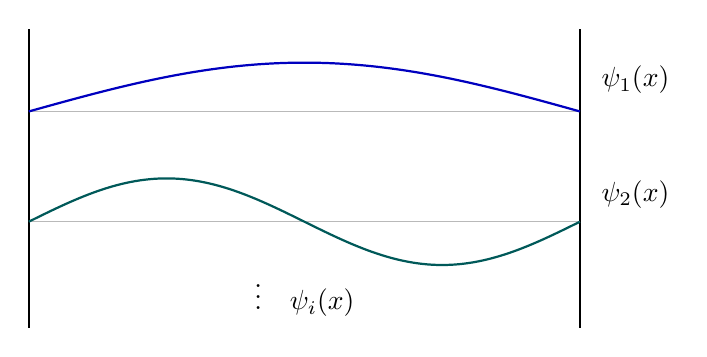
\begin{tikzpicture}[x=1cm,y=1cm]
  \draw[thick] (0,0) -- (0,3.8);
  \draw[thick] (7,0) -- (7,3.8);
  \draw[gray!55] (0,2.75) -- (7,2.75);
  \draw[gray!55] (0,1.35) -- (7,1.35);
  \draw[blue!75!black,thick,domain=0:7,samples=120]
    plot (\x,{2.75+0.62*sin(180*\x/7)});
  \draw[teal!70!black,thick,domain=0:7,samples=120]
    plot (\x,{1.35+0.55*sin(360*\x/7)});
  \node[right] at (7.15,3.15) {$\psi_1(x)$};
  \node[right] at (7.15,1.70) {$\psi_2(x)$};
  \node at (3.5,0.45) {$\vdots\quad \psi_i(x)$};
\end{tikzpicture}
\caption{A clean reconstruction of the qualitative box-mode sketch. The vertical displacement separates the eigenfunctions for readability and is not an additional physical coordinate.}
\end{figure}

The index \(i\) labels a one-particle state, not a particle and not the number of nodes. For the box basis, \(i\) happens to be one more than the number of interior nodes. Each state has an energy \(\varepsilon_i\). Following the lecture's notation we may write this energy as \(\hbar\omega_i\), or simply \(\omega_i\) after setting \(\hbar=1\).

\begin{classroomqa}
\lecturetimestamp{00:39:01}
\audiencequestion{Was the earlier independence assumption exact, and could the index \(i\) label the possible states of an electron in an atom?}
\lecturerresponse{For the independent-mode construction the commutation between different modes is exact. The index may label one-particle atomic states. If the particles interact, however, the simple independent-mode Hamiltonian is no longer the whole story.}
\end{classroomqa}

\begin{classroomqa}
\lecturetimestamp{00:40:34}
\audiencequestion{Is the particle in the box a boson?}
\lecturerresponse{It may be, but with one particle the statistics do not matter. Exclusion and exchange become meaningful only when there is more than one identical particle.}
\end{classroomqa}

\section{From Box Modes to Fock Space}

Now allow any number of identical bosons in the box. Some number \(n_1\) may occupy \(\psi_1\), some number \(n_2\) may occupy \(\psi_2\), and so on. A basis state is therefore
\begin{equation}
|n_1,n_2,n_3,\ldots\rangle.
\end{equation}
This is exactly the notation already used for many oscillators. The identity is structural: associate one oscillator with every one-particle state, and identify the oscillator excitation number with the number of particles occupying that state.

Bosons are essential here because every \(n_i\) may be any nonnegative integer. For fermions each one-particle state can be empty or singly occupied, never doubly occupied, so the ordinary oscillator algebra cannot be used unchanged.

The operators can now be defined by their action on the occupation-number basis. The operator \(a_i^\dagger\) creates one particle in one-particle state \(i\); \(a_i\) removes one:
\begin{align}
a_i^\dagger|n_1,\ldots,n_i,\ldots\rangle
&=\sqrt{n_i+1}\,|n_1,\ldots,n_i+1,\ldots\rangle, \\
a_i|n_1,\ldots,n_i,\ldots\rangle
&=\sqrt{n_i}\,|n_1,\ldots,n_i-1,\ldots\rangle.
\end{align}
This is not an analogy after the fact. It is the definition of the bosonic creation and annihilation operators on this basis. Because the basis spans the space, the definition determines their action on every state by linearity.

\begin{classroomqa}
\lecturetimestamp{00:47:11}
\audiencequestion{Are \(n_1,n_2,n_3\) the quantum states?}
\lecturerresponse{The labels \(1,2,3,\ldots\) identify the one-particle states. The symbols \(n_1,n_2,n_3,\ldots\) are the numbers of particles occupying those states. Keeping the state label and its occupation number distinct is the main notational burden.}
\end{classroomqa}

\subsection{What the square root does}

The factor \(\sqrt{n_i+1}\) does not represent an additional particle or a separate physical process. It gives the operator the correct normalization and algebra. In one mode,
\begin{align}
a a^\dagger|n\rangle
&=a\bigl(\sqrt{n+1}\,|n+1\rangle\bigr) \\
&=(n+1)|n\rangle,
\end{align}
while
\begin{equation}
a^\dagger a|n\rangle=n|n\rangle.
\end{equation}
Their difference is therefore \(|n\rangle\), as required by \([a,a^\dagger]=1\). The two ladder operators are, very roughly, each of order \(\sqrt n\), since their product gives the number operator of order \(n\).

\begin{classroomqa}
\lecturetimestamp{00:47:52}
\audiencequestion{What tangible physical meaning belongs to the square-root factor?}
\lecturerresponse{It is primarily mathematical normalization. It ensures that the occupation states are normalized, that \(a^\dagger a\) has eigenvalue \(n\), and that the ladder operators obey the oscillator commutator. Sometimes the mathematics is the meaning one needs.}
\end{classroomqa}

\begin{classroomqa}
\lecturetimestamp{00:52:25}
\audiencequestion{Have the creation and annihilation operators been defined only through their properties and their action on the basis?}
\lecturerresponse{Yes. Definitions need not arise from a more primitive picture. Their value is tested by their consequences. Defining the action on a complete basis defines the operators everywhere, and these definitions reproduce the desired commutation relations.}
\end{classroomqa}

\begin{classroomqa}
\lecturetimestamp{00:53:22}
\audiencequestion{Why does \(a_i\) make a particle disappear rather than merely move it to a different state?}
\lecturerresponse{Because \(a_i\) is defined to lower the occupation of state \(i\). The useful question is not why a definition is true, but why it is useful. It is useful because emission and absorption require operators that change particle number: a photon is created when radiation is emitted and annihilated when it is absorbed.}
\end{classroomqa}

The space spanned by all occupation-number states is \emph{Fock space}. It contains the vacuum, every one-particle state, every two-particle state, and so on without a fixed upper bound:
\begin{equation}
\mathcal F=\mathcal H_0\oplus\mathcal H_1\oplus\mathcal H_2\oplus\cdots.
\label{eq:l06-fock-space}
\end{equation}
The direct-sum notation makes explicit what the ordinary \(N\)-particle wavefunction did not: all particle-number sectors belong to one state space.

\begin{classroomqa}
\lecturetimestamp{00:54:56}
\audiencequestion{Does defining the operators on the occupation-number eigenvectors determine them on arbitrary vectors, and do the oscillator commutators then follow?}
\lecturerresponse{Exactly. The occupation vectors form a basis, so linearity extends the definition to all of Fock space. Acting on that basis verifies the bosonic commutation relations. Each one-particle state is represented by one oscillator, and its oscillator occupation is the number of particles in that state.}
\end{classroomqa}

\subsection{The vacuum and the free Hamiltonian}

The Fock vacuum is the state with no particles in any one-particle state:
\begin{equation}
|0\rangle=|0,0,0,\ldots\rangle,
\qquad a_i|0\rangle=0.
\end{equation}
The word \emph{ground state} can be misleading here. The lowest \emph{one-particle} state is the mode \(i=1\); the Fock vacuum has no particle even in that mode. If a particle occupies the lowest mode, \(a_1\) can remove it and return the system to the vacuum.

\begin{classroomqa}
\lecturetimestamp{00:56:19}
\audiencequestion{What is the vacuum in occupation-number language? Is the lowest one-particle state occupied?}
\lecturerresponse{The vacuum has every occupation number equal to zero and is annihilated by every \(a_i\). The lowest one-particle mode is unoccupied in the vacuum. If it were occupied, its annihilation operator could remove that particle.}
\end{classroomqa}

For noninteracting particles, the total energy is additive. If one particle in state \(i\) has energy \(\hbar\omega_i\), then
\begin{align}
H
&=\sum_i \hbar\omega_i N_i \\
&=\sum_i \hbar\omega_i a_i^\dagger a_i.
\label{eq:l06-free-fock-hamiltonian}
\end{align}
There are two equivalent readings. It is the sum of oscillator energies, one oscillator per one-particle state. It is also the sum over one-particle energies, each multiplied by the number of particles carrying that energy.

In field-theory notation \(a_i^\dagger\) is usually called the creation operator and \(a_i\) the annihilation operator. The older \(a_+\) and \(a_-\) notation says the same thing.

\section{Clarifications Before the Field Appears}

Several questions after the break separate the new oscillator bookkeeping from an ordinary particle moving in an oscillator potential.

\begin{classroomqa}
\lecturetimestamp{01:06:09}
\audiencequestion{The energy levels of a particle in a box are not equally spaced, so where is the harmonic oscillator?}
\lecturerresponse{The one-particle energies \(\omega_i\) need not be equally spaced. For each fixed mode \(i\), however, the energies of zero, one, two, and three noninteracting particles in that mode are \(0,\omega_i,2\omega_i,3\omega_i\). That occupation ladder is the oscillator. It is distinct from putting one particle in a harmonic-oscillator potential.}
\end{classroomqa}

\begin{classroomqa}
\lecturetimestamp{01:08:38}
\audiencequestion{Is this construction connected with Fourier decomposition?}
\lecturerresponse{Deeply. If the one-particle basis consists of momentum modes, the mode functions are sines, cosines, or complex exponentials, and the \(a_i\) are quantum analogues of Fourier coefficients. A general basis need not be trigonometric, but the expansion logic is the same.}
\end{classroomqa}

\begin{classroomqa}
\lecturetimestamp{01:09:07}
\audiencequestion{Are all particles being assigned the same energy, and are interactions included?}
\lecturerresponse{Particles occupying the same one-particle state have the same energy, while particles in different states generally do not. For now the particles are free: they do not interact. Interactions would add potential-energy terms, so the Hamiltonian would no longer be only the additive sum in Equation~\eqref{eq:l06-free-fock-hamiltonian}.}
\end{classroomqa}

\begin{classroomqa}
\lecturetimestamp{01:10:26}
\audiencequestion{What became of the half quantum of zero-point energy in every oscillator?}
\lecturerresponse{It is an additive constant in the Hamiltonian. A constant commutes with every operator, so it does not alter Heisenberg equations of motion, and ordinary nongravitational measurements depend on energy differences. It may matter for special purposes, but it does not affect the construction being developed here.}
\end{classroomqa}

The free theory is already a bookkeeping device of unusual power. It keeps track not only of many particles but of particles that change state, appear, disappear, or exist in superpositions of different total number. The operators are more than bookkeeping symbols because suitable Hermitian combinations can be measured, but bookkeeping is a useful first intuition.

\begin{classroomqa}
\lecturetimestamp{01:14:03}
\audiencequestion{Where did field theory and quantum field theory come from historically?}
\lecturerresponse{A brief historical route begins with Faraday's physical picture of electric and magnetic fields and Maxwell's equations for classical fields. Planck introduced energy quanta while studying thermal radiation; Einstein identified the quantization with the electromagnetic field itself and with light quanta. Heisenberg, Pauli, and especially Dirac then helped put the modern operator framework together around the end of the 1920s. The ultraviolet catastrophe and the quantum description of radiation were among the decisive early problems. This is a schematic history rather than a complete assignment of priority.}
\end{classroomqa}

The historical thread also explains why oscillators keep returning. Classical radiation in a cavity decomposes into normal modes. Quantizing those modes turns their excitation numbers into photon numbers. The mathematical quanta occupying the modes become physical particles.

\section{The Bosonic Field Operator}

Let \(\{\psi_i(x)\}\) be a complete orthonormal basis of one-particle wavefunctions. Define
\begin{equation}
\boxed{\Psi(x)=\sum_i a_i\,\psi_i(x)}
\label{eq:l06-field-annihilation}
\end{equation}
and its Hermitian conjugate
\begin{equation}
\boxed{\Psi^\dagger(x)=\sum_i a_i^\dagger\,\psi_i^*(x)}.
\label{eq:l06-field-creation}
\end{equation}

\begin{figure}[htbp]
\centering

\includegraphics[width=0.9\linewidth]{lecture_06_frame_04.png}
\caption{The completed mode expansions of the annihilation field and its Hermitian conjugate. Equations~\eqref{eq:l06-field-annihilation} and \eqref{eq:l06-field-creation} preserve the same operator and complex-conjugation structure in typeset form.}
\lectureframe{01:25:15}
\end{figure}

For any fixed position \(x\), each \(\psi_i(x)\) is an ordinary complex number. All operator content resides in \(a_i\) and \(a_i^\dagger\). As \(x\) varies, we obtain a different operator at every point in space. This is the precise sense in which \(\Psi\) is an operator-valued function.

If the basis functions are plane waves, Equations~\eqref{eq:l06-field-annihilation} and \eqref{eq:l06-field-creation} are quantum Fourier expansions: the classical Fourier coefficients have become operators. In a box, the basis may instead be the sine functions in Equation~\eqref{eq:l06-box-basis}. Any complete orthonormal one-particle basis works.

Neither \(\Psi\) nor \(\Psi^\dagger\) is Hermitian. Observable fields can be built from Hermitian combinations such as
\begin{equation}
\Psi(x)+\Psi^\dagger(x),
\qquad
i\bigl(\Psi^\dagger(x)-\Psi(x)\bigr),
\end{equation}
and observable densities will later be built from products such as \(\Psi^\dagger(x)\Psi(x)\). The present task is first to understand what the two basic fields do.

\begin{classroomqa}
\lecturetimestamp{01:23:14}
\audiencequestion{How can the left side be an operator when the mode functions on the right are ordinary wavefunctions?}
\lecturerresponse{The functions \(\psi_i(x)\) are numbers once \(x\) is chosen. The factors \(a_i\) are operators. A number times an operator is an operator, and the sum is therefore an operator. Varying \(x\) gives the whole family of operators.}
\end{classroomqa}

\section{What the Field Does}

The annihilation field kills the vacuum immediately:
\begin{equation}
\Psi(x)|0\rangle
=\sum_i\psi_i(x)a_i|0\rangle
=0.
\label{eq:l06-field-kills-vacuum}
\end{equation}
The creation field does something much more informative.

Let \(|i\rangle\) denote the one-particle state with wavefunction
\begin{equation}
\langle x|i\rangle=\psi_i(x).
\end{equation}
Completeness of the one-particle basis gives
\begin{equation}
\sum_i|i\rangle\langle i|=1.
\label{eq:l06-completeness}
\end{equation}
Apply this identity to a position eigenstate:
\begin{align}
|x\rangle
&=\sum_i|i\rangle\langle i|x\rangle \\
&=\sum_i\psi_i^*(x)|i\rangle.
\label{eq:l06-position-expansion}
\end{align}
In Fock language a one-particle mode state is
\begin{equation}
|i\rangle=a_i^\dagger|0\rangle.
\end{equation}
Substituting this in Equation~\eqref{eq:l06-position-expansion},
\begin{align}
|x\rangle
&=\sum_i\psi_i^*(x)a_i^\dagger|0\rangle \\
&=\Psi^\dagger(x)|0\rangle.
\label{eq:l06-local-creation}
\end{align}
Thus \(\Psi^\dagger(x)\) creates a particle localized at \(x\), while \(\Psi(x)\) removes one there. A position eigenstate is delta-function localized and is a generalized, non-normalizable state; a physical localized particle is obtained by smearing the field with a normalizable wavepacket.\editorialnote{The lecture speaks in the ideal position-eigenstate language. The wavepacket qualification records the standard mathematical meaning without changing the argument.}

\begin{classroomqa}
\lecturetimestamp{01:36:26}
\audiencequestion{Where is the information specifying what kind of particle is created? Is the state at \(x\) delta-function localized?}
\lecturerresponse{A separate field is assigned to each particle species, so the identity of the particle is carried by which field is used. The argument \(x\) specifies where it is created. In the ideal position basis, the created state has delta-function localization.}
\end{classroomqa}

Examples of bosonic species include photons, gravitons, Higgs bosons, and gluons, though realistic fields also carry internal indices. Even photons require polarization labels. The simplified scalar field notation suppresses those extra labels so that the creation principle remains visible.

\subsection{The vacuum is not the zero vector}

The equation
\begin{equation}
\Psi(x)|0\rangle=0
\end{equation}
contains two very different objects denoted by zero. The ket \(|0\rangle\) is the vacuum: a normalized physical state with
\begin{equation}
\langle0|0\rangle=1.
\end{equation}
The result on the right is the zero vector. Its norm is zero; it cannot be normalized and does not represent a physical state.

The difference becomes sharp under addition. Adding the zero vector to a one-particle state changes nothing. Adding the vacuum to a one-particle state gives a genuine superposition of different particle-number sectors. With normalized coefficients,
\begin{equation}
|\chi\rangle=\frac{1}{\sqrt2}\bigl(|0\rangle+|1\rangle\bigr)
\end{equation}
has equal probabilities for zero and one particle. It is not the same as \(|1\rangle\).

\begin{classroomqa}
\lecturetimestamp{01:37:23}
\audiencequestion{If no particle is present at \(x\), does \(\Psi(x)\) simply do nothing? What does it mean for the result to be zero?}
\lecturerresponse{It does not return the original state. It returns the zero vector. The vacuum is a normalized state describing empty space; the zero vector has zero length and describes no physical state. Any operator acting on the zero vector returns the zero vector.}
\end{classroomqa}

\begin{classroomqa}
\lecturetimestamp{01:39:00}
\audiencequestion{What happens if the vacuum rather than the zero vector is added to a one-particle state?}
\lecturerresponse{One obtains a superposition with amplitudes for different particle numbers. By contrast, adding the zero vector leaves the one-particle state unchanged. The symbol in \(|0\rangle\) names zero occupation; it does not mean zero vector.}
\end{classroomqa}

\begin{classroomqa}
\lecturetimestamp{01:41:56}
\audiencequestion{Does the order of a mode function and its creation or annihilation operator matter in the field expansion? Are the mode functions complex?}
\lecturerresponse{The mode function is an ordinary number and therefore commutes with every operator, so the order does not matter. In general the mode functions may be complex; whether a chosen basis is real or complex depends on the one-particle Schr\"odinger problem.}
\end{classroomqa}

\subsection{Two particles and the emergence of bosonic symmetry}

To create one particle at \(x\) and another at \(y\), act twice:
\begin{equation}
|x,y\rangle
=\Psi^\dagger(y)\Psi^\dagger(x)|0\rangle.
\label{eq:l06-two-particle-state}
\end{equation}
The points may coincide or differ. Since the underlying creation operators commute,
\begin{align}
[\Psi^\dagger(x),\Psi^\dagger(y)]
&=\sum_{i,j}\psi_i^*(x)\psi_j^*(y)
[a_i^\dagger,a_j^\dagger] \\
&=0.
\end{align}
It follows that
\begin{equation}
\Psi^\dagger(y)\Psi^\dagger(x)|0\rangle
=\Psi^\dagger(x)\Psi^\dagger(y)|0\rangle.
\label{eq:l06-boson-exchange}
\end{equation}
Exchanging the order of the two particles changes nothing. This is precisely bosonic exchange symmetry. We could therefore have started from the oscillator algebra and \emph{derived} that the particles constructed from commuting creation operators are bosons. Fermions will require anticommuting operators instead.

\begin{classroomqa}
\lecturetimestamp{01:42:37}
\audiencequestion{How is a second particle added to the one-particle state?}
\lecturerresponse{Apply another creation field. To add it at \(y\), act with \(\Psi^\dagger(y)\) to the left of \(\Psi^\dagger(x)\). The result is the two-particle state in Equation~\eqref{eq:l06-two-particle-state}.}
\end{classroomqa}

\begin{classroomqa}
\lecturetimestamp{01:46:04}
\audiencequestion{Is the commutativity of the two creation fields fully equivalent to symmetrizing the two-particle state?}
\lecturerresponse{Yes. It makes the state with one particle at \(x\) and one at \(y\) identical to the state obtained after exchanging the labels. This is the defining exchange property of identical bosons.}
\end{classroomqa}

\begin{classroomqa}
\lecturetimestamp{01:46:32}
\audiencequestion{Does this mean the particles at \(x\) and \(y\) must be the same kind of boson?}
\lecturerresponse{Yes. The arguments \(x\) and \(y\) are positions, while one field describes one species. Different species, and additional labels such as the two photon polarizations, require distinct field components.}
\end{classroomqa}

\section{Why Variable Particle Number Matters}

If a problem contained exactly thirty-seven particles forever, the field language would be optional bookkeeping. Its real strength appears when particles can be emitted and absorbed, and especially when particle number itself is a quantum variable. Fock space allows states of the form
\begin{equation}
|\Phi\rangle
=c_0|0\rangle+c_1|1\rangle+c_2|2\rangle+\cdots,
\qquad
\sum_{n=0}^{\infty}|c_n|^2=1.
\end{equation}
A laser field is an important example: it is not generally a state with one sharp photon number, but a superposition of many number sectors.

The bridge between particles and fields is now explicit. The mode operators count and change particles in energy eigenstates; the field combines those operators with a complete set of wavefunctions so that particles can be created or removed at specified positions. The algebra of harmonic oscillators has become the elementary language of a bosonic quantum field.
